\section{Thermodynamik}
\subsection{Die Zustandsgrößen}
Thermodynamische Systeme (viele Freiheitsgrade)
\begin{figure}[H]
    \begin{center}
        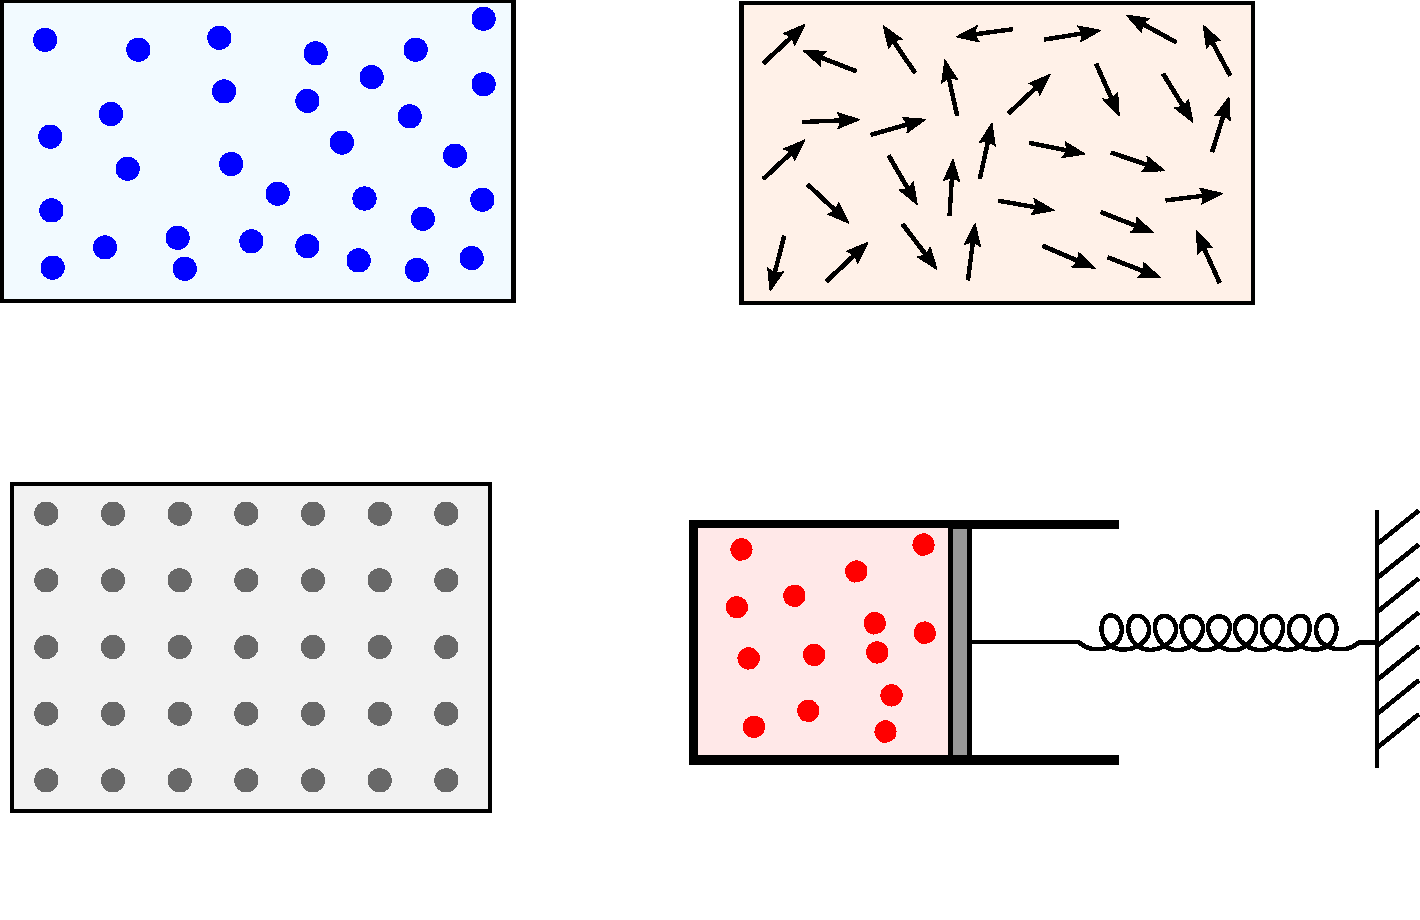
\includegraphics[width=\textwidth]{../img/exampleSystems.pdf}
        \caption{Beispiele komplizierter thermodynamischer Systeme (Gasgefäß, Kolben Feder)}
        \label{img:exampleSystems}
    \end{center}
\end{figure}
Es gibt zwei Arten von thermodynamischen Systemen:
\begin{enumerate}
    \item abgeschlossene Systeme
    \item offene Systeme
\end{enumerate}
Thermodynamische (Zustands-)größen:
Apparativ messbare Eigenschaften des Systems (relevante Größen)
\begin{equation}
    p, V, E, T, S, N, \mu, \vec{M}, \vec{H}, c_p, \ldots
\end{equation}
\begin{itemize}
    \item extensive Variable (proportional zu Menge des Systems)
    \begin{equation}
        V, E, S, \vec{M}, N
    \end{equation}
    \item intensive Variable (unabhängig von der Menge des Systems)
    \begin{equation}
        p, T, \rho=\frac{N}{V}, \vec{H}
    \end{equation}
\end{itemize}
Thermodynamisches Gleichgewicht: Keine zeitliche Änderung der thermodynamischen Größen
\subsection{0. Hauptsatz der Thermodynamik}
$A$ im Gleichgewicht mit $B$ und $B$ im Gleichgewicht mit $C \Rightarrow A$ im Gleichgewicht mit $C$ \\
Beziehungen zwischen den Zustandsgrößen: \\
Beispiel: Ideales Gas (einatomig)
\begin{equation}
    \begin{split}
        p V &= N k T \\
        E &= \frac{3}{2} N k T
    \end{split}
\end{equation}
mit $k=k_\text{Boltzmann} \approx 1.38\cdot 10^{-23}\,\frac{\text{J}}{\text{K}}$ \\
Zustandsgrößen mit \emph{mechanischer} Signifikanz:
\begin{equation}
    $E, V, N, M$ \qquad \text{(sind auch für ein Teilchen definiert)}
\end{equation}
Ideales Gas:
\begin{equation}
    \begin{split}
        p &= \frac{2}{3} \frac{E}{V} \\
        k T &= \frac{2}{3} \frac{E}{N}
    \end{split}
\end{equation}
\subsection{1. Hauptsatz der Thermodynamik}
Innere Energie $E$:
\begin{equation}
    \begin{split}
        E&=\const \quad \text{(abgeschlossenes System)} \\
        \difd E &= \delta A + \delta Q \quad \text{(offenes System)}
    \end{split}
\end{equation}
Die innere Energie ist eine Zustandsgröße.
\begin{description}
    \item[$\delta A$] kontrollierte Energiezufuhr durch adiabatische (sehr langsame) Änderung von mechanischen Parametern.
    \item[$\delta Q$] unkontrollierte Energiezufuhr
\end{description}
\subsubsection{Beispiele für $\delta Q$}
\begin{enumerate}[a)]
    \item $\delta Q = m g \Delta h$
    \begin{figure}[H]
        \begin{center}
            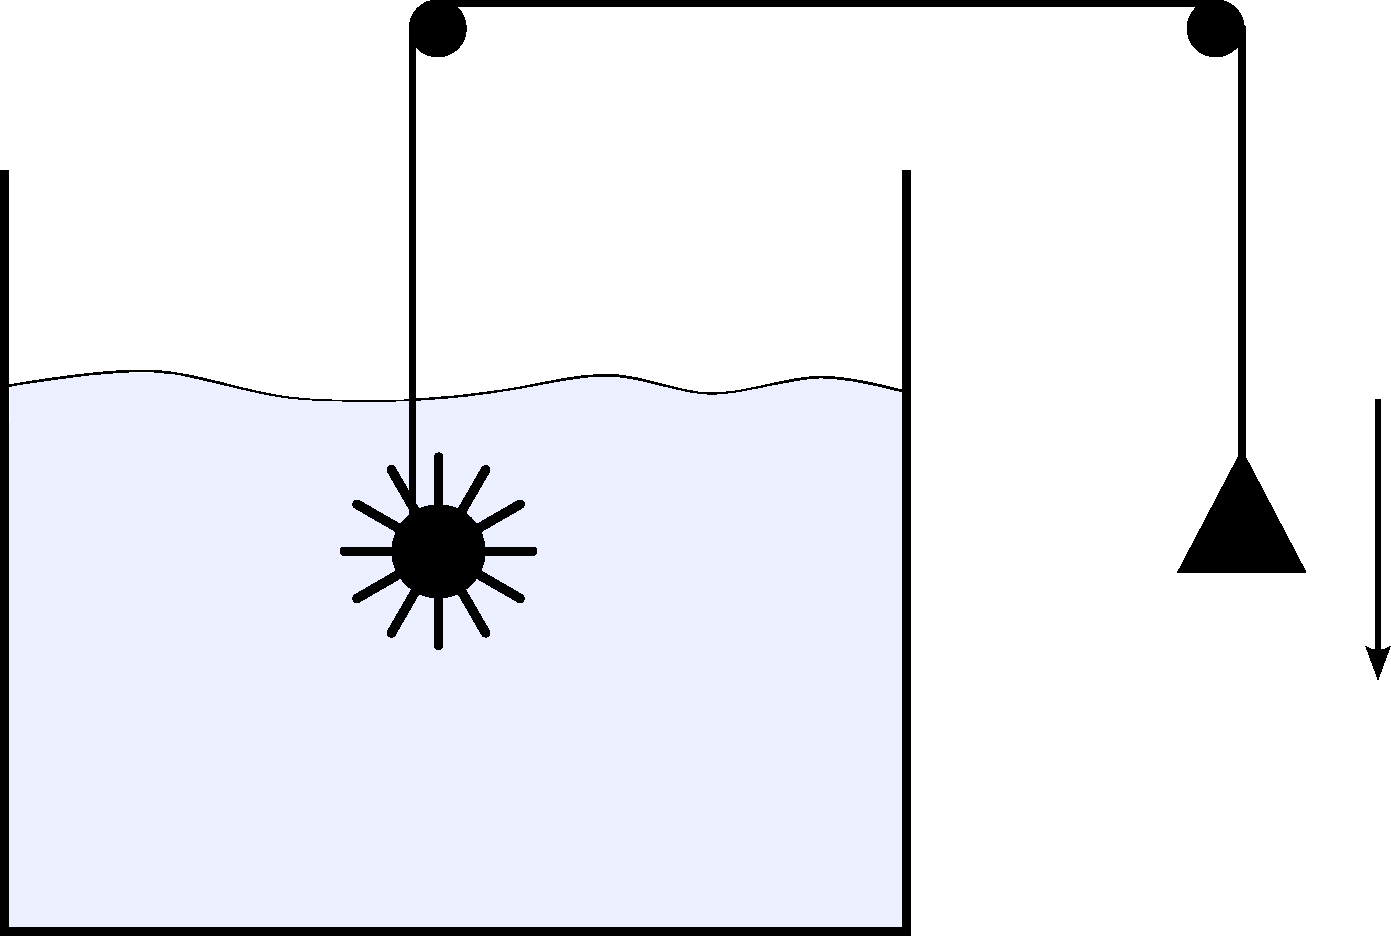
\includegraphics[width=0.3\textwidth]{../img/exampleDQpot.pdf}
            \caption{caption}  % TODO label
            \label{img:exampleDQpot}
        \end{center}
    \end{figure}
    
    \item  $\delta Q = I^2 R \delta t$
    \begin{figure}[H]
        \begin{center}
            \includegraphics[width=0.3\textwidth]{../img/exampleDQinductor.pdf}
            \caption{caption}  % TODO label
            \label{img:exampleDQcoil}
        \end{center}
    \end{figure}
\end{enumerate}
\subsubsection{Beispiele für $\delta A$}
\begin{enumerate}[a)]
    \item
    \begin{equation}
        \delta A = k \difd x = p F \difd x = - p \difd V
    \end{equation}
    \begin{figure}[H]
        \begin{center}
            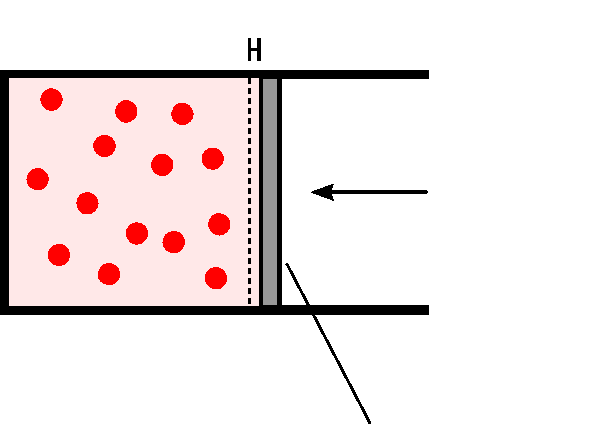
\includegraphics[width=0.3\textwidth]{../img/exampleDApiston.pdf}
            \caption{Kolben.}  % TODO label
            \label{img:exampleDApiston}
        \end{center}
    \end{figure}
    \item Magnetisierung, Magnetfeld
    \begin{equation}
        k = M \frac{\difd H'}{\difd x}
    \end{equation}
    \begin{figure}[H]
        \begin{center}
            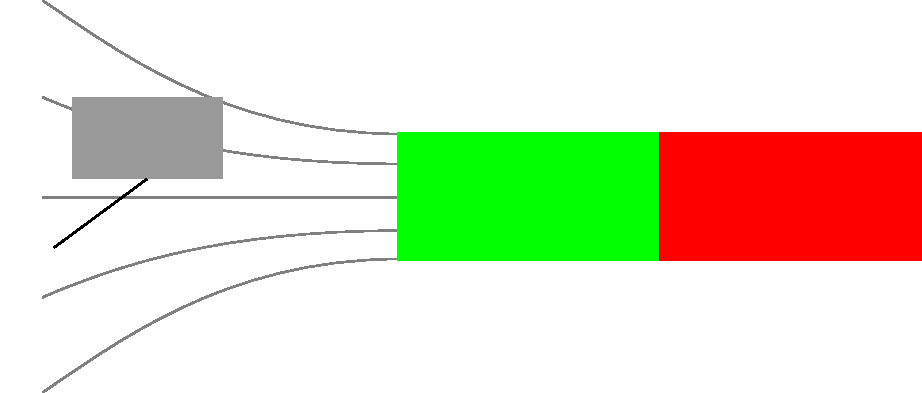
\includegraphics[width=0.3\textwidth]{../img/exampleDAmagnetism.pdf}
            \caption{Magnetisierung.}  % TODO label
            \label{img:exampleDAmagnetism}
        \end{center}
    \end{figure}
    \begin{enumerate}[i)]
        \item Magnetisierung der Probe
        \begin{equation}
            -A_1 = \int K \difd x \int M \frac{\difd H'}{\difd x} \difd x = \int_{0}^{H} M \difd H'
        \end{equation}
        \item Magnetisierung des Feldes bei fester Magnetisierung
        \begin{equation}
            - A_2 = M(H) \int_{H}^{0} \difd H' = - M(H) \cdot H^0
        \end{equation}
    \end{enumerate}
    Gesamtheit der Magnetisierung $A = A_1 + A_2$
    \begin{equation}
        \begin{split}
            \delta A &= \delta A_1 + \delta A_2 = - M \difd H + \difd(M \cdot H) \\
            &= - M \difd H + H \difd M + M \difd H \\
            &= H \difd M
        \end{split}
    \end{equation}
    Nicht-inifitesimale Arbeit:
    \begin{figure}[H]
        \begin{center}
            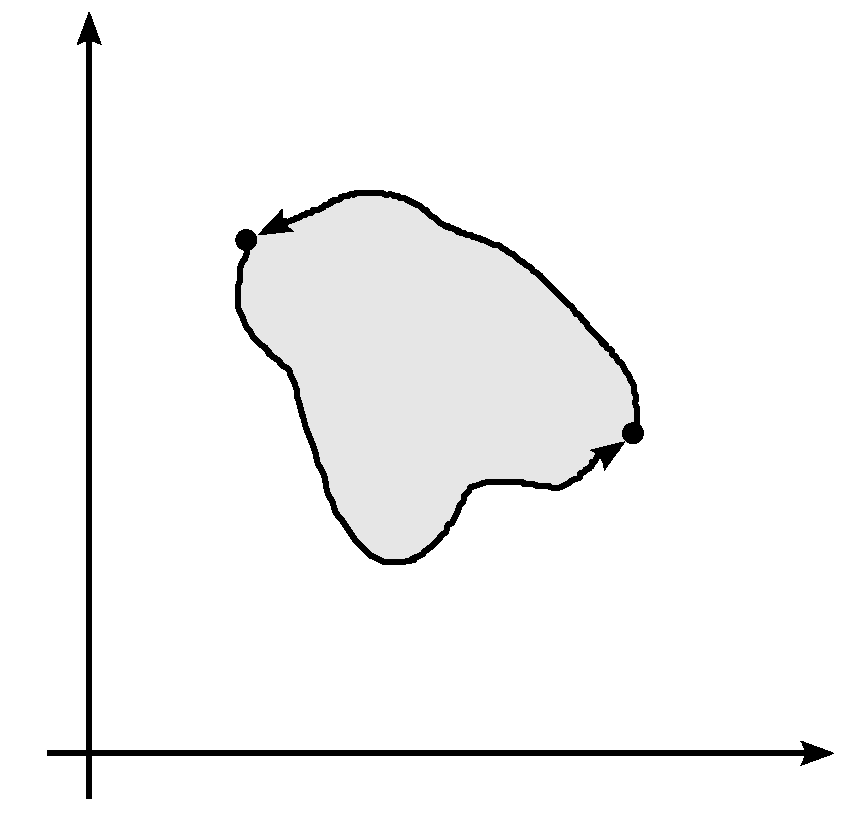
\includegraphics[width=0.49\textwidth]{../img/notInfWork_p-V.pdf}
            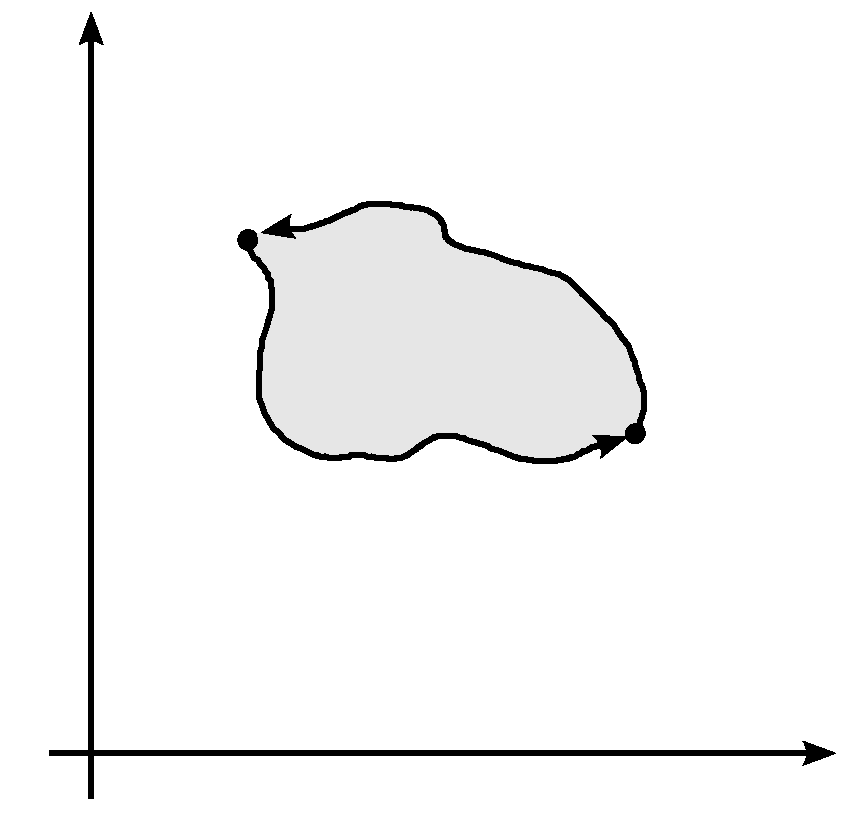
\includegraphics[width=0.49\textwidth]{../img/notInfWork_H-M.pdf}
            \caption{Nicht-inifitesimale Arbeit.}  % TODO label
            \label{img:label}
        \end{center}
    \end{figure}
    \begin{equation}
        A_{pV} = - \oint p \difd V \text{  (Fläche)} \qquad \qquad \qquad A_{HM} = - \oint H \difd M \text{  (Fläche)}
    \end{equation}
    Nun beachte: Die Arbeit ist \emph{keine} Zustandsgröße, da Wegabhängigkeit.
    \begin{equation}
        - \int_\mathcal{W} p \difd V \neq - \int_\mathcal{V} p \difd V
    \end{equation}
    \begin{figure}[H]
        \begin{center}
            \includegraphics[width=0.3\textwidth]{../img/pathsWV_in_p-V.pdf}
            \caption{Zwei Wege $\mathcal{W}$ und $\mathcal{V}$ im $p$-$V$-Diagram.}
            \label{img:pathsVW_in_p-V}
        \end{center}
    \end{figure}
    
    \paragraph{Exkurs über vollständige (totale) Differentiale}
    \begin{equation}
        \begin{split}
            F(x, y) \Rightarrow \difd F &= \underbrace{\pd{F}{x}}_{A(x, y)} \difd x + \underbrace{\pd{F}{y}}_{B(x, y)} \difd y \\
            &= A(x, y) \difd x + B(x, y) \difd y
        \end{split}
    \end{equation}
    Man beachte: $A$ und $B$ sind nicht unabhängig! \\
    z.B. gilt
    \begin{equation}
        \pd{A}{y} = \frac{\partial^2 F}{\partial y \partial x} = \frac{\partial^2 F}{\partial x \partial y} = \pd{B}{x}
    \end{equation}
    Für eine beliebige Form $\delta \Phi = C(x, y) \difd x + D(x, y) \difd y$ gilt:
    \begin{equation}
        \delta \Phi \text{ totales Differential } \Leftrightarrow \pd{C}{y} = \pd{D}{x}
    \end{equation}
    Weiterhin gilt:
    \begin{equation}
        \int \delta \Phi \text{ wegunabhängig} \Leftrightarrow \delta \Phi \text{ totales Differential}
    \end{equation}
    Beispiel:
    \begin{equation}
        \begin{split}
            & \delta A = - p \difd V = - p \difd V + 0 \difd p \\
            & \Rightarrow
            \begin{cases}
                C = - p \\
                D = 0
            \end{cases}
            \Rightarrow \pd{C}{p} = -1 \neq 0 = \pd{D}{V}
        \end{split}
    \end{equation}
    d.h. $\delta A$ ist \emph{kein} totales Differential. \\[\baselineskip]
    Verallgemeinerung zu mehreren Dimensionen und Beispiele : Übungsgruppen \\
    Insbesondere für $\delta \Phi = \sum_i a_i (x_1, \ldots, x_\nu) \difd x_i$ gilt:
    \begin{equation}
        \int \delta \Phi \text{ wegunabhängig} \Leftrightarrow \pd{a_i}{x_j} = \pd{a_j}{x_i} \quad \forall i, j
    \end{equation}
    \item Allgemeine, kontrollierbare Arbeitsänderung
    \begin{figure}[H]
        \begin{center}
            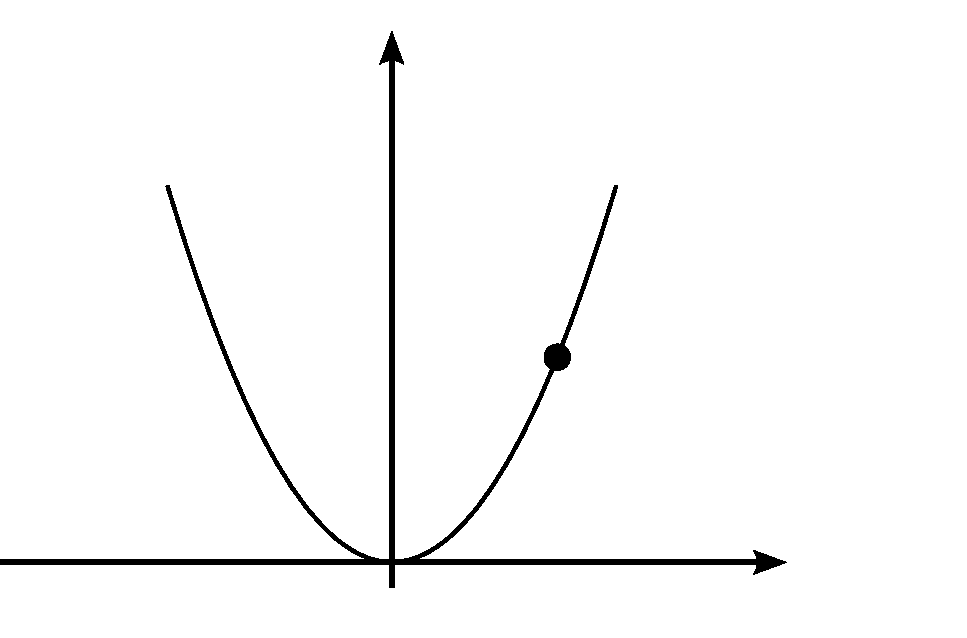
\includegraphics[width=0.3\textwidth]{../img/controlledDeltaWork.pdf}
            \caption{caption}  % TODO caption
            \label{img:controlledDeltaWork}
        \end{center}
    \end{figure}
    Äußere Parameter $E(x_1, \ldots, x_n)$ \\
    Verallgemeinerte Kraft:
    \begin{equation}
        K_i = - \pd{E}{x_i}
    \end{equation}
\end{enumerate}
\subsubsection{Adiabatensatz}
(z.B. Landau-Lifschitz §11) \\
Eine sehr langsame (quasistatische) Änderung von $x$ produziert keine Wärme ($\delta Q = 0$). Damit ist 
\begin{equation}
    \difd E = - \sum_i K_k \difd x_i
\end{equation}
Allgemein:
\begin{equation}
    \difd E = \delta Q - \sum_i K_i \difd x_i \qquad \text{(1. Hauptsatz)}
\end{equation}

\subsection{2. Hauptsatz der Thermodynamik}
\begin{figure}[H]
\begin{center}
  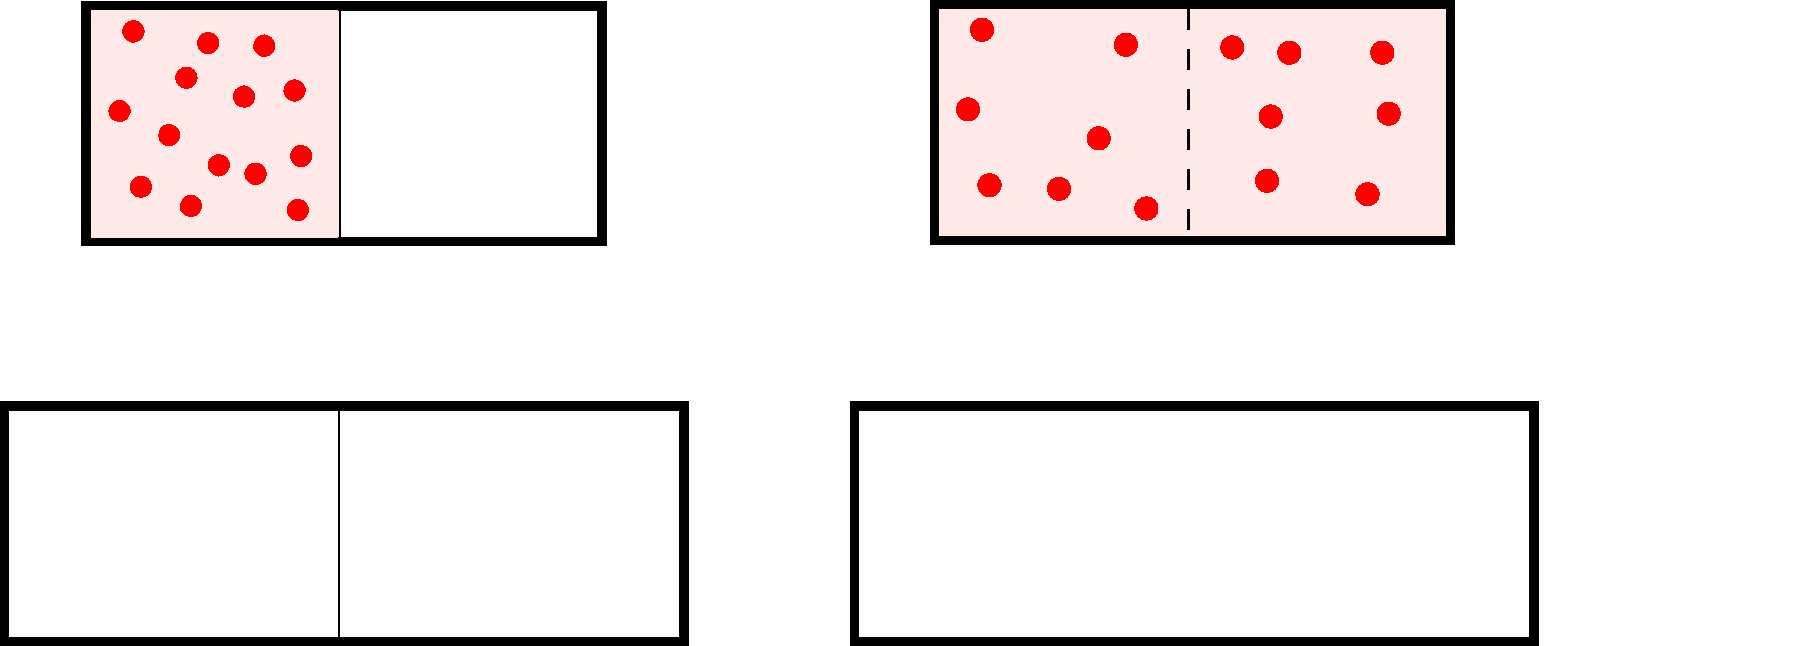
\includegraphics[width=0.5\textwidth]{../img/irrevProcess.pdf}
  \caption{caption}  % TODO caption
  \label{img:irrevProcess}
\end{center}
\end{figure}
Irreversible Prozesse, Ablauf?
\begin{enumerate}[a)]
    \item Es gibt eine extensive Zustandsgröße $S(E, V, N, \ldots)$, die \emph{Entropie}, die den Ablauf von Prozessen regelt.
    \item In einem abgeschlossenen System kann die Entropie nicht abnehmen. $S$ ist ein Maß für die Unordnung
    (Unschärfe der Kenntnis über den mikroskopischen Zustand)
\end{enumerate}

\subsubsection{Äquivalente Formulierung des 2. Hauptsatzes}
(Es gibt kein \emph{perpetuum mobile} 2. Art) \\
Es gibt keine periodisch arbeitende Maschine, die \emph{ausschließlich}
\begin{enumerate}[I.]
    \item Wärme aus einem kalten in ein wärmeres Reservoir überführt (\textsc{Clausius})
    \item Wärme in Arbeit umwandelt (\textsc{Thomson}, \textsc{Lord Kelvin})
\end{enumerate}
\paragraph{Folgerungen}
\begin{itemize}
    \item aus b): für ein abgeschlossenes System gilt
    \begin{equation}
        \difd S = 0 \qquad
        \begin{cases}
            \text{i) } & \difd S > 0 \Leftrightarrow \text{Prozess irreversibel} \\
            \text{ii)} & \difd S = 0 \Leftrightarrow \text{Prozess reversibel}
        \end{cases}
    \end{equation}
    \item Thermodynamisches Gleichgewicht: $S$ maximal unter Berücksichtigung der gegebenen Randbedingungen
\end{itemize}
Die Entropie ist die zentrale statistische Größe der Thermodynamik und der statistischen Physik. Sie ist eine \emph{nicht-mechanische} Größe.
Alle anderen nicht-mechanischen Größen ($\delta Q, T, \ldots$) können aus $S$ hergeleitet werden.
\subsubsection{Die Temperatur}
\begin{figure}[H]
    \begin{center}
        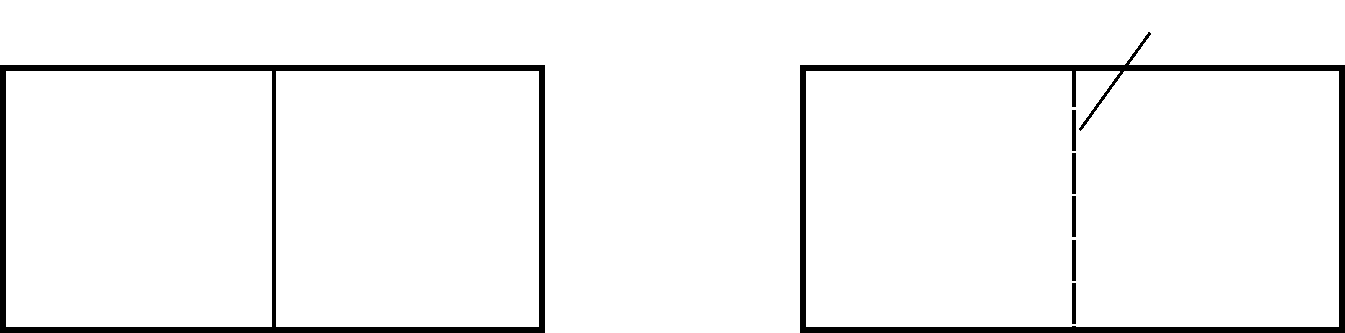
\includegraphics[width=0.3\textwidth]{../img/derivationT.pdf}
        \caption{caption}  % TODO caption
        \label{img:derivationT}
    \end{center}
\end{figure}
\begin{equation}
    \label{eq:derivationT:constTotEnergy}
	\difd E_1 = - \difd E_2 \qquad \text{(konstante Gesamtenergie)}
\end{equation}
\begin{equation}
    S = S_1(E_1, V_1, N_1) + S_2 (E_2, V_2, N_2)
\end{equation}
Im Gleichgewicht:
\begin{equation}
    \label{eq:derivationT:equilibrium}
    0 = \difd S = \pd{S_1(E_1, V_1, N_1)}{E_1} \difd E_1 + \pd{S_2 (E_2, V_2, N_2)}{E_2} \difd E_2
\end{equation}
Mit \autoref{eq:derivationT:constTotEnergy} und \autoref{eq:derivationT:equilibrium} folgt:
\begin{equation}
    \pd{S_1}{E_1} = \pd{S_2}{E_2} =: \frac{1}{T} \qquad T:\text{absolute Temperatur}
\end{equation}

\paragraph{Eichung} Tripelpunkt des Wassers
\begin{figure}[H]
\begin{center}
  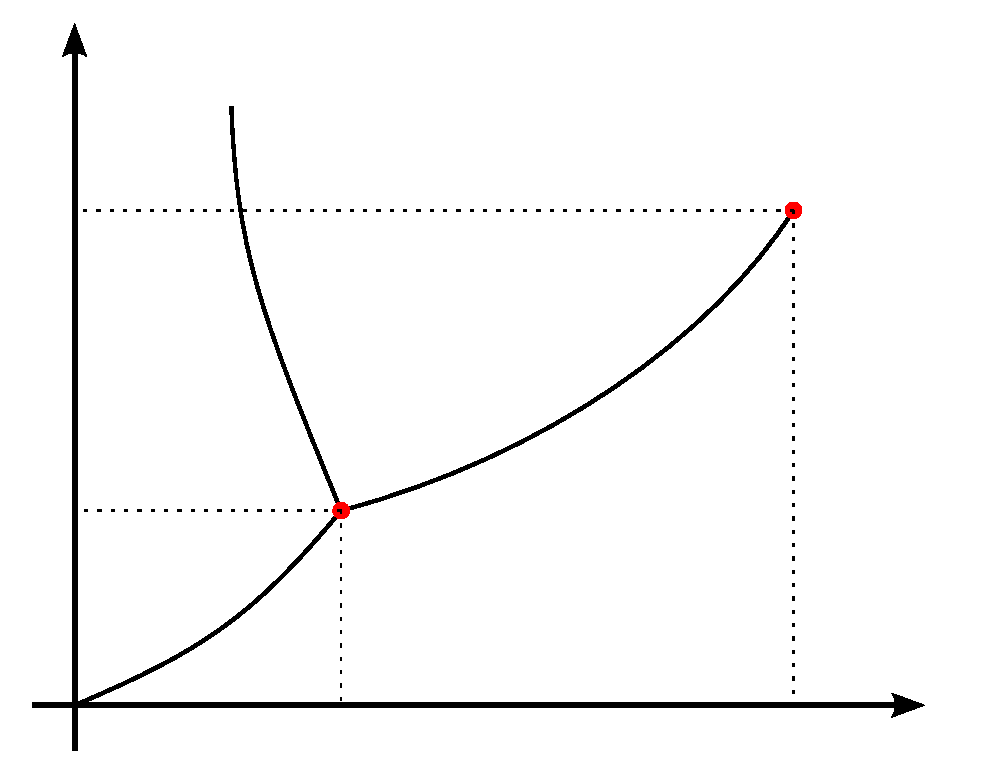
\includegraphics[width=0.3\textwidth]{../img/tripelpoint.pdf}
  \caption{Tripelpunkt des Wassers.}
  \label{img:tripelpoint}
\end{center}
\end{figure}
\begin{equation}
    \begin{split}
        T_t &= 273.16 \, \text{K} \qquad P_t = 611.7 \, \text{Pa} \\
        T_t &= 647.36 \, \text{K} \qquad P_t = 22.06 \, \text{MPa}
    \end{split}
\end{equation}

\paragraph{Richtung des Energieflusses} \mbox{}\\ 
Im Gleichgewicht: $T_1 = T_2$ \\
Richtung des Energieflusses bei $T_1 \neq T_2$ ?
\begin{equation}
    \begin{split}
        & \pd{S_1}{E_1} = \frac{1}{T_1}, \qquad \pd{S_2}{E_2} = \frac{1}{T_2} \\
        & 0 < \difd S = \frac{1}{T_1} \difd E_1 + \frac{1}{T_2} \difd E_2 = \left( \frac{1}{T_1} - \frac{1}{T_2} \right) \difd E_1
    \end{split}
\end{equation}
$\Rightarrow$ für $T_2 > T_1$ ist $\difd E_1 > 0$. \\
Es ist:
\begin{equation}
    \frac{\difd E}{\difd t} \propto (T_2 - T_1) \qquad \text{(empirisch)}
\end{equation}
\begin{equation}
    \Rightarrow \frac{\difd S}{\difd t} \propto \frac{(T_2 - T_1)^2}{T_1 T_2}
\end{equation}
d.h. \emph{Entropieproduktion} ist proportional zu $(T_2 - T_1)^2$. Wichtig bei Fluktuationen, bei irreversibler Thermodynamik.

\subsubsection{Die Wärme(menge)}
\begin{equation}
    \difd S_1 = \frac{1}{T_1} \difd E_1 \overset{(*)}{=} \frac{1}{T_1} \delta Q
\end{equation}
$(*)$: Energietransfer ohne Arbeitsleistung
\begin{equation}
    \Rightarrow \delta Q = T \difd S \qquad \text{2. Hauptsatz}
\end{equation}
\subsubsection{Der Druck}
\begin{figure}[H]
    \begin{center}
        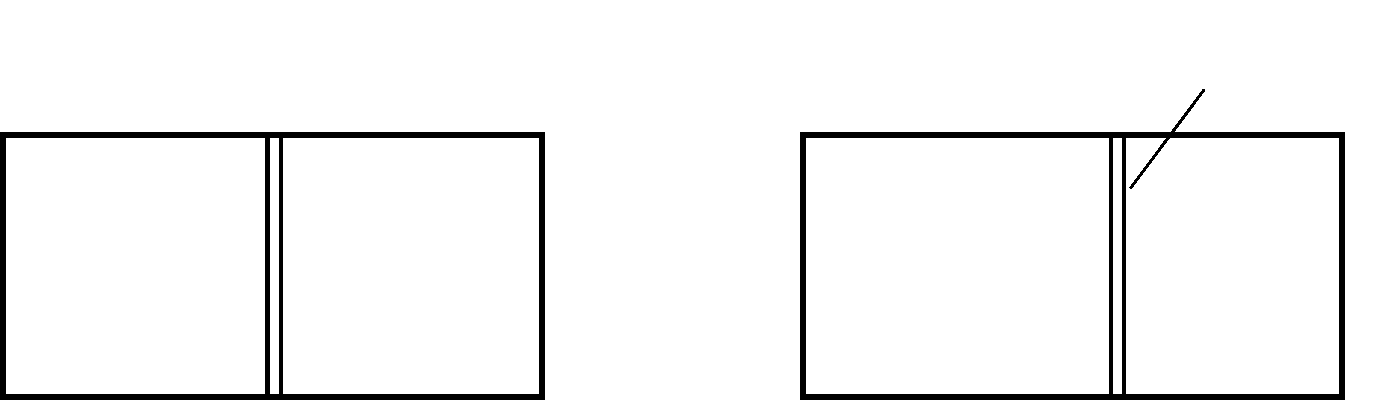
\includegraphics[width=0.3\textwidth]{../img/derivationP.pdf}
        \caption{caption}  % TODO caption
        \label{img:derivatoinP}
    \end{center}
\end{figure}
\begin{equation}
    \begin{split}
        & \difd E_1 = - \difd E_2 \\
        & \difd V_1 = - \difd V_2 \\
        & \difd S_1 = \pdi{S_1}{E_1}{V_1, N_1} \difd E_1 + \pdi{S_1}{V_1}{E_1, N_1} \difd V_1 \\
        & \Rightarrow \difd E_1 = \underbrace{T_1 \difd S_1}_{\delta Q_1} - \underbrace{T_1 \pdi{S_1}{V_1}{E_1, N_1}}_{p_1 \text{ (Äquivalenzbet.; 1. HS.)}} \difd V_1
    \end{split}
\end{equation}
\begin{equation}
    \Rightarrow p = T \pdi{S}{V}{E, N}
\end{equation}
Gleichgewicht: Volumenaustausch und Wärmeaustausch
\begin{equation}
    \begin{split}
        & \difd V_1 = - \difd V2, \qquad \difd E_1 = - \difd E_2 \\
        & \Rightarrow \difd S = \left( \frac{1}{T_1} - \frac{1}{T_2} \right) \difd E_1 + \left( \frac{p_1}{T_1} - \frac{p_2}{T_2} \right) \difd V_1
    \end{split}
\end{equation}
Im Gleichgewicht: $\difd S = 0$
\begin{equation}
    \Rightarrow T_1 = T_1 , \qquad p_1 = p_2
\end{equation}
\subsubsection{Das chemische Potential}
\begin{figure}[H]
    \begin{center}
        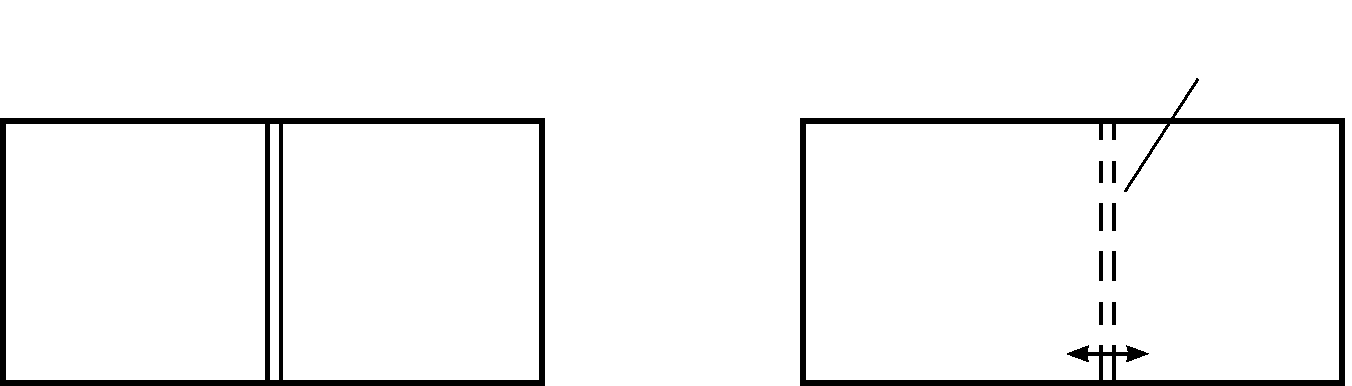
\includegraphics[width=0.3\textwidth]{../img/derivationMu.pdf}
        \caption{caption}  % TODO caption
        \label{img:derivationMu}
    \end{center}
\end{figure}
Energie-, Volumen- und Teilchenaustausch.
\begin{equation}
    \begin{split}
        \difd S_1 &= \pdi{S_1}{E_1}{V_1, N_1} \difd E_1 + \pdi{S_1}{V_1}{E_1, N_1} \difd V_1 + \pdi{S_1}{N_1}{E_1, V_1} \difd N_1 \\
        & \Rightarrow \difd E_1 = \underbrace{T_1 \difd S_1}_{\delta Q} - \underbrace{p_1 \difd V_1}{\text{mech. Arbeit}}
        \underbrace{- T_1 \pdi{S_1}{N_1}{E_1, V_1}}_{\mu_1} \difd N1
    \end{split}
\end{equation}
$\mu$: Chemisches Potential
\begin{equation}
    \Rightarrow E_1 = \delta Q_1 - p_1 \difd V_1 + \mu_1 \difd N_1
\end{equation}
\begin{equation}
    \mu = - T_1 \pdi{S_1}{N_1}{E_1, V_1}
\end{equation}
Im Gleichgewicht, wie oben, folgt $\mu_1 = \mu_2$.

\subsubsection{Fundamentale Gleichung}
\begin{equation}
    \label{eq:fundamentalEQ}
    \difd E = T \difd S - p \difd V + \mu \difd N
\end{equation}
$E(S, V, N)$ ist eine Funktion von \emph{extensiven} Variablen.

\subsubsection{Anwendungsbeispiele}
\begin{enumerate}
    \item Entropie des idealen Gases (einatomig) \\
    Konstante Teilchenzahl $N$
    \begin{equation}
        \begin{split}
            & T \difd S = \difd E + p \difd V, \qquad p V = N k T, \qquad E = \frac{3}{2} N k T \\
            & \Rightarrow \difd S = \frac{\difd E}{T} + \frac{p}{T} \difd V = \frac{3}{2} N k \frac{\difd E}{E} + N k \frac{\difd V}{V}
        \end{split}
    \end{equation}
    $\difd S$ totales Differential:
    \begin{equation}
        \Rightarrow S - S_0 = \frac{3}{2} N k \ln (\frac{E}{E_0}) + N k \ln (\frac{V}{V_0})
    \end{equation}
    Bemerkung: $S$ extensiv (korrekt!), da Ausdruck proportional zu $N$.
    \paragraph{Adiabate} Linien konstanter Entropie \\
    Hier: $\ln(E^{3/2} V) = \const \Leftrightarrow E^{3/2} V = \const$ \\
    Äquivalente Schreibweise: $T^{3/2} V = \const \Leftrightarrow p^{3/2} V^{3/2} V = \const$ \\
    $\Leftrightarrow p^{3/2} V^{5/2} = \const \Leftrightarrow p V^{5/3} = \const$
    \begin{figure}[H]
        \begin{center}
            \includegraphics[width=\textwidth]{../img/adiabate_pV_ST.pdf}
            \caption{caption}  % TODO caption
            \label{img:adiabate_pV_ST}
        \end{center}
    \end{figure}
    \item Gleichheit der absoluten Temperatur $T$ und der Temperatur des idealen Gases $T_G$
    Denkbar ist $T_G = f(T)$
    \begin{equation}
        \begin{split}
            & \difd S = \frac{1}{T} \difd E + \frac{p}{T}\difd V \qquad \text{Integrabilitätsbedingung} \\
            & \frac{\partial}{\partial E} \left( \frac{p}{T} \right)_V = \frac{\partial}{\partial V} \left( \frac{1}{T} \right)_E = 0 \quad \text{da } E = \frac{3}{2} N k T_G
        \end{split}
    \end{equation}
    Ideales Gas: $p V = N k T_G$
    \begin{equation}
        \begin{split}
            \Rightarrow & \frac{\partial}{\partial E} \left( \frac{p}{T} \right)_V = \frac{N k }{V} \frac{\partial}{\partial E} \left( \frac{T_G}{T} \right)_V = 0 \\
            \Rightarrow & \frac{\partial}{\partial T_G} \left( \frac{T_G}{T} \right) = 0 \\
            \Rightarrow & T_G = T \cdot \const
        \end{split}
    \end{equation}
    Die Konstante wird durch den Tripelpunkt des Wassers fixiert.
    \item \emph{Wirkungsgrad} einer Wärmekraftmaschine
    \begin{figure}[H]
        \begin{center}
            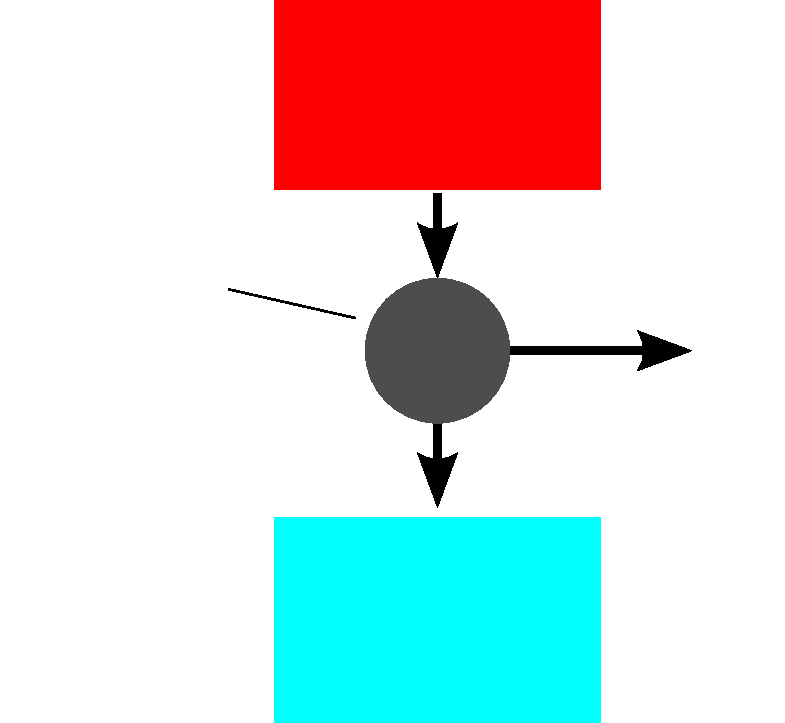
\includegraphics[width=0.3\textwidth]{../img/waermekraftmaschine.pdf}
            \caption{Wärmekraftmaschine.}
            \label{img:waermekraftmaschine}
        \end{center}
    \end{figure}
    
    \begin{figure}[H]
        \begin{center}
            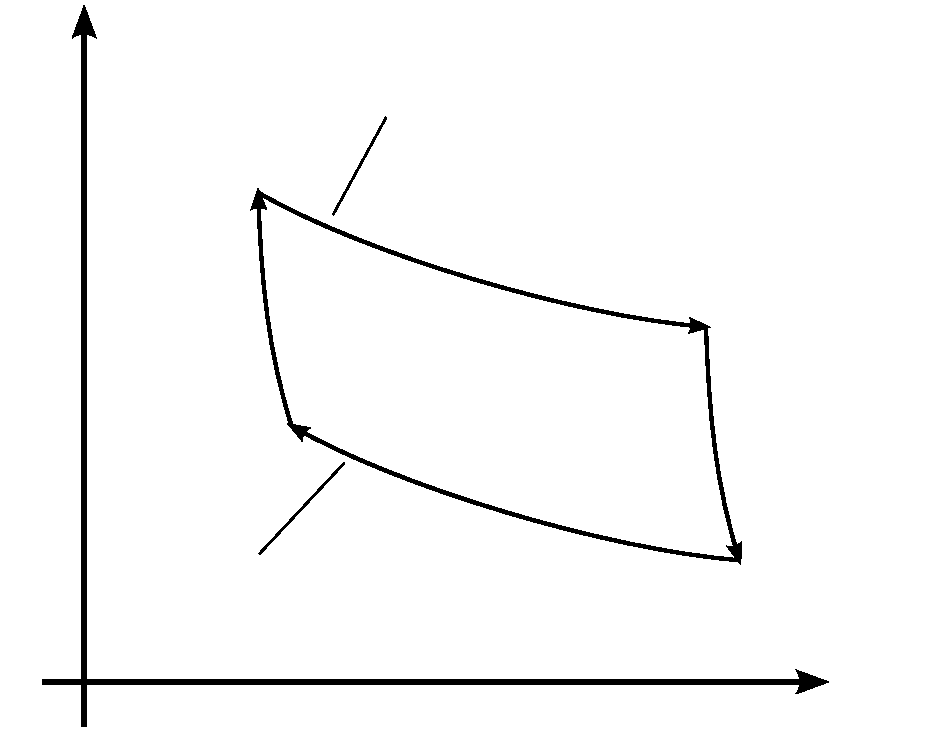
\includegraphics[width=0.3\textwidth]{../img/carnotprocess.pdf}
            \caption{Carnot-Prozess.}
            \label{img:carnot}
        \end{center}
    \end{figure}
    
    Reversibel:
    \begin{equation}
        \begin{split}
            & \Delta S = 0 \Rightarrow - \frac{Q_2}{T_2} + \frac{Q_1}{T_1} + 0  \\
            & \Rightarrow \frac{Q_2}{T_2} = \frac{Q_1}{T_1} = \gamma
        \end{split}
    \end{equation}
    Energieerhaltung (Maschine soll nach \emph{Zyklus} im Ausgangszustan sein $\Rightarrow A = Q_2 - Q_1$) \\
    Wirkungsgrad $\eta$:
    \begin{equation}
        \eta := \frac{A}{Q_2} \Rightarrow \eta_{\text{reversibel}} = \frac{Q_2 - Q_1}{q_2} = \frac{T_2 - T_1}{T_2}
    \end{equation}
    Wärmepumpe:
    \begin{equation}
        \bar{\eta} = \frac{Q_1}{A} (\text{für } T_1 > T_2) \Rightarrow \bar{\eta}_{\text{reversibel}} = \frac{T_1}{T_1 - T_2}
    \end{equation}
    Kühlmaschine:
    \begin{equation}
        \bar{\bar{\eta}} = \frac{Q_2}{-A} (\text{für } T_1 > T_2) \Rightarrow \bar{\bar{\eta}}_{\text{reversibel}} = \frac{T_2}{T_1-T_2}
    \end{equation}
    irreversibel:
    \begin{equation}
        \Delta S > 0 \Rightarrow \frac{Q_1'}{T_1} > \frac{Q_2'}{T_2}
    \end{equation}
    Wirkungsgrad der Wärmekraftmaschine: $\eta_{\text{irrev.}} = \frac{A'}{Q_2'}$ \\
    Sei z.B. $Q_2' = Q_2 \Rightarrow Q_1' > Q_1$
    \begin{equation}
        \begin{split}
            \Rightarrow & A' = Q_2' - Q_1' = Q_2 - Q_1' < A \\
            \Rightarrow & \eta_\text{irrev.} < \eta_\text{reversibel}
        \end{split}
    \end{equation}
    Wirkungsgrad der idealen \emph{Carnot-Maschine} ist maximal.
\end{enumerate}

\subsection{Einige Folgerungen aus den Hauptsätzen}
\subsubsection{Wichtige abgeleitete Größen}
\begin{itemize}
    \item Spezifische Wärme
    \begin{equation}
        \begin{split}
            c_p &= \left( \frac{\Delta Q}{\Delta T} \right)_p = T \left( \frac{\partial S}{\partial T} \right)_p \\
            c_V &= \left( \frac{\Delta Q}{\Delta T} \right)_p = T \left( \frac{\partial S}{\partial T} \right)_V
        \end{split}
    \end{equation}
    Technische Definition bezogen auf 1 Mol, $N=N_A$ (Avogadro) \\
    Korrekterweise: $s = \frac{S N_A}{N}, \quad v = \frac{V N_A}{N}$, siehe Adam + Hittmair \\
    hier sehen wir davon ab
    \item Kompressibilität
    \begin{equation}
        \begin{split}
            \kappa_s &= - \frac{1}{V} \left( \frac{\partial V}{\partial p} \right)_S \text{ (adiabatisch)} \\
            \kappa_T &= - \frac{1}{V} \left( \frac{\partial V}{\partial p} \right)_T \text{ (isotherm)}
        \end{split}
    \end{equation}
    \item Ausdehnungskoeffizient
    \begin{equation}
        \alpha = \frac{1}{V} \left( \frac{\partial V}{\partial T} \right)_p
    \end{equation}
    \item Magnetische Suszeptibilität
    \begin{equation}
        \chi = \left( \frac{\partial M}{\partial H} \right)_T
    \end{equation}
\end{itemize}
Diese Größen sind der Messung direkt zugänglich. Man beachte: die verschiedenen Größen sind nicht unabhängig, z.B. gilt
$c_p - c_v = V T \alpha^2 / \kappa_T$ (Beweis später).
Woher kommen diese Abhängigkeiten? \emph{Integrabilitätsbeziehungen}!
\subsubsection{Maxwell-Beziehungen}
Fundamentale Gleichung \eqref{eq:fundamentalEQ}:
\begin{equation}
    \difd E = T \difd S - p \difd V + \mu \difd N, \quad E=E(S, V, N)
\end{equation}
\paragraph{Freie Energie} $F:=E - TS$ (\textsc{Legendre}-Transformation)
\begin{equation}
    \begin{split}
        \Rightarrow & \difd F = \difd E - T \difd S - S \difd T \\
        \Rightarrow & \difd F = -S\difd T - p \difd V + \mu \difd N \\
        \Rightarrow & F=F(T, V, N)
    \end{split}
\end{equation}
\paragraph{Enthalpie} $H:=E+pV$
\begin{equation}
    \begin{split}
        \Rightarrow & \difd H = \difd E + p \difd V + V \difd p \\
        \Rightarrow & \difd H = T \difd S + V \difd p + \mu \difd N \\
        \Rightarrow & H=H(S, p, N)
    \end{split}
\end{equation}
\paragraph{Freie Enthalpie} $G:=E-T+pV$
\begin{equation}
    \begin{split}
        \Rightarrow & \difd G = - S \difd T + V \difd p + \mu \difd N \\
        \Rightarrow & G=G(T, p, N)
    \end{split}
\end{equation}
$E, F, H, G$ heißen \emph{Thermodynamische Potentiale}.
\paragraph{Integrabilitätsbeziehungen} \mbox{}\\
aus $E$:
\begin{equation}
    \left( \frac{\partial T}{\partial V} \right)_{S, N} = \left( \frac{\partial p}{\partial S} \right)_{V, N}, \quad
    \left( \frac{\partial T}{\partial N} \right)_{S, V} = \left( \frac{\partial \mu}{\partial S} \right)_{V, N}, \quad
    - \left( \frac{\partial p}{\partial N} \right)_{S, V} = \left( \frac{\partial \mu}{\partial V} \right)_{S, N}
\end{equation}
aus $F$:
\begin{equation}
    \left( \frac{\partial S}{\partial V} \right)_{T, N} = \left( \frac{\partial p}{\partial T} \right)_{V, N}, \quad \text{usw.}
\end{equation}
aus $H$:
\begin{equation}
    \left( \frac{\partial T}{\partial p} \right)_{S, N} = \left( \frac{\partial V}{\partial S} \right)_{p, N}, \quad \text{usw.}
\end{equation}
aus $G$:
\begin{equation}
    - \left( \frac{\partial S}{\partial p} \right)_{T, N} = \left( \frac{\partial V}{\partial T} \right)_{p, N}, \quad \text{usw.}
\end{equation}
\textsc{Maxwell}-Beziehungen (insgesamt 12 Beziehungen)
\subsubsection{Exkurs: Variablentransformation}
Erwünscht:
\begin{equation}
    \left( \frac{\partial E}{\partial V} \right)_T \overset{?}{\rightarrow} \left( \frac{\partial E}{\partial V} \right)_p
    \text{ oder }
    \left( \frac{\partial E}{\partial V} \right)_T \overset{?}{\rightarrow} \left( \frac{\partial E}{\partial p} \right)_T
\end{equation}
Wichtig: Jacobi'sche Determinanten $f=f(x, y)$; $g=g(x, y)$ \\
Definition:
\begin{equation}
    \frac{\partial (f, g)}{\partial(x, y)} = \det
    \begin{pmatrix}
\frac{\partial f}{\partial x} & \frac{\partial f}{\partial y} \\
\frac{\partial g}{\partial x} & \frac{\partial g}{\partial y}
\end{pmatrix}
= \left( \frac{\partial f}{\partial x} \right) \left( \frac{\partial g}{\partial
y} \right) - \left( \frac{\partial f}{\partial y} \right) \left( \frac{\partial g}{\partial x} \right)
\end{equation}
Rechenregeln
\begin{equation}
    \frac{\partial(f, g)}{\partial(x, y)} = -\frac{\partial(f, g)}{\partial(y, x)}; \qquad
    \frac{\partial(f, y)}{\partial(x, y)} = \frac{\partial f}{\partial x}
\end{equation}
und für $x=(u, v), y=(u, v)$
\begin{equation}
    \Rightarrow \frac{\partial(f, g)}{\partial(u, v)} = \frac{\partial(f, g)}{\partial(x, y)} \cdot \frac{\partial(x, y)}{\partial(u, v)}
\end{equation}
Beweis:
\begin{equation}
    \begin{split}
        \det
        \begin{pmatrix}
\frac{\partial f}{\partial u} & \frac{\partial f}{\partial v} \\
\frac{\partial g}{\partial u} & \frac{\partial g}{\partial v}
\end{pmatrix}
&= \det \left[
\begin{pmatrix}
\frac{\partial f}{\partial x} & \frac{\partial f}{\partial y} \\
\frac{\partial g}{\partial x} & \frac{\partial g}{\partial y}
\end{pmatrix}
\cdot
\begin{pmatrix}
\frac{\partial x}{\partial u} & \frac{\partial x}{\partial v} \\
\frac{\partial y}{\partial u} & \frac{\partial y}{\partial v}
\end{pmatrix}
\right] \\
&= \det
\begin{pmatrix}
\frac{\partial f}{\partial x} & \frac{\partial f}{\partial y} \\
\frac{\partial g}{\partial x} & \frac{\partial g}{\partial y}
\end{pmatrix}
\cdot \det
\begin{pmatrix}
\frac{\partial x}{\partial u} & \frac{\partial x}{\partial v} \\
\frac{\partial y}{\partial u} & \frac{\partial y}{\partial v}
\end{pmatrix} \qquad \square
    \end{split}
\end{equation}
Spezialfall der Kettenregel:
\begin{equation}
    \frac{\partial(f, g)}{\partial(x, y)} \cdot \frac{\partial(x, y)}{\partial(f, g)} = 1
\end{equation}
\subsubsection{Anwendungsbeispiele} $N$ = konstant
\begin{enumerate}  % a), b)
    \item
    \begin{equation}
        \begin{split}
            c_p &=  T \left( \frac{\partial S}{\partial T} \right)_p = T \frac{\partial(S, p)}{\partial(T, p)} \overset{\text{$V$ abh.}}{=}
            T \frac{\partial(S, p)}{\partial(T, V)} / \underbrace{\frac{\partial(T, p)}{\partial(T, V)}}_{ \left( \frac{\partial p}{\partial V} \right)_T} \\
            &= \frac{T}{ \left( \frac{\partial p}{\partial V} \right)_T} \left[ \left( \frac{\partial S}{\partial T} \right)_V
            \left( \frac{\partial p}{\partial V} \right) - \left( \frac{\partial S}{\partial V} \right)_T \left( \frac{\partial p}{\partial T} \right)_V \right] \\
            &= c_V - T \left( \frac{\partial S}{\partial V} \right)_T \left( \frac{\partial p}{\partial T} \right)_V / \left( \frac{\partial p}{\partial V} \right)_T \\
            &\overset{\text{Maxwell-Bez.}}{=} c_V - T \left( \frac{\partial p}{\partial T} \right)_V^2 / \left( \frac{\partial p}{\partial V} \right)_T
        \end{split}
    \end{equation}
    Nun ist
    \begin{equation}
        \begin{split}
            \left( \frac{\partial p}{\partial T} \right)_V &= \frac{\partial(p, V)}{\partial (T, V)} \\
            &= \frac{\partial (p, V)}{\partial (p, T)} \cdot \frac{\partial(p, T)}{\partial(T, V)} \\
            &= \left( \frac{\partial V}{\partial T} \right)_p \cdot \left[ - \left( \frac{\partial p}{\partial V} \right)_T \right]
        \end{split}
    \end{equation}
    \begin{equation}
        \Rightarrow c_p = c_V - T \left( \frac{\partial V}{\partial T} \right)_p^2 \left( \frac{\partial p}{\partial V} \right)_T = c_V + T V \alpha^2 / \kappa_T^2
    \end{equation}
    \item
    \begin{equation}
        \frac{c_p}{c_v} = \frac{\kappa_T}{\kappa_S} \quad \text{(Übungsaufgabe)}
    \end{equation}
\end{enumerate}
\subsubsection{Die Gibbs-Duhem-Beziehung}
Fundamentalgleichung (\autoref{eq:fundamentalEQ}), $E, S, V, N$ sind extensive Variablen
\begin{equation}
    \difd E = T \difd S - p \difd V + \mu \difd N
\end{equation}
Somit gilt für $E=E(S, V, N)$ dass $E(\alpha S, \alpha V, \alpha N) = \alpha E(S, V, N)$ (homogene Funktion nach \textsc{Euler})
\paragraph{Eulerscher Satz über homogene Funktion} $f(x_1, \ldots, x_n)$: \\
Falls $f(\alpha x_1, \ldots, \alpha x_n) = \alpha^r f(x_1, \ldots, x_n)$ so ist
\begin{equation}
    \sum_{i=1}^{n} x_i \frac{\partial f}{\partial x_i} = r f
\end{equation}
Beweis: Differentiation nach $\alpha$ und dann $\alpha = 1$ setzten.
\paragraph{Fundamentalrelation}\mbox{}\\
Damit folgt
\begin{equation}
    \begin{split}
        E &= \left( \frac{\partial E}{\partial S} \right)_{V, N} S + \left( \frac{\partial E}{\partial V} \right)_{S, N} V + \left( \frac{\partial E}{\partial N} \right)_{V, S} N \\
        &= T S - p V + \mu N
    \end{split}
\end{equation}
Damit, im Gleichgewicht
\begin{equation}
    E = T S - p V + \mu N \qquad \text{Fundamentalrelation}
\end{equation}
Differentiation ergibt:
\begin{equation}
    \difd E = T \difd S + S \difd T - p \difd V - V \difd P + \mu \difd N + N \difd \mu
\end{equation}
\begin{equation}
    \Rightarrow S \difd T - V \difd p + N \difd \mu = 0 \qquad \text{\textsc{Gibbs-Duhem} Beziehung}
\end{equation}
D.h. $T$, $p$ und $\mu$ nicht unabhängig voneinander. \\
Folgerung: Die Zustandsgleichung muss zur eindeutigen Charakterisierung des Systems zumindest \emph{eine} extensive Größe enthalten. \\
Folgerungen für die thermodynamischen Potentiale:
\begin{equation}
    \begin{split}
        & E(S, V, N) = T S - p V + \mu N \\
        & F(T, V, N) = E - TS = - pV + \mu N \\
        & H(S, p, N) = E + p V = T S + \mu N \\
        & G(T, p, N) = E + p V - T S = \mu N
    \end{split}
\end{equation}
Man beachte: obwohl $G=\mu N$ recht einfach erscheint, ist zur Kennzeichnung des Systems die Kenntnis von $\mu$ als Funktion der \emph{natürlichen}
Variablen $T, p, N$, d.h. die Funktionalität $\mu(T, p, N)$ notwendig.

\subsubsection{Der Joule-Thomson-Prozess (gedrosselte Entspannung)}
\begin{figure}[H]
\begin{center}
  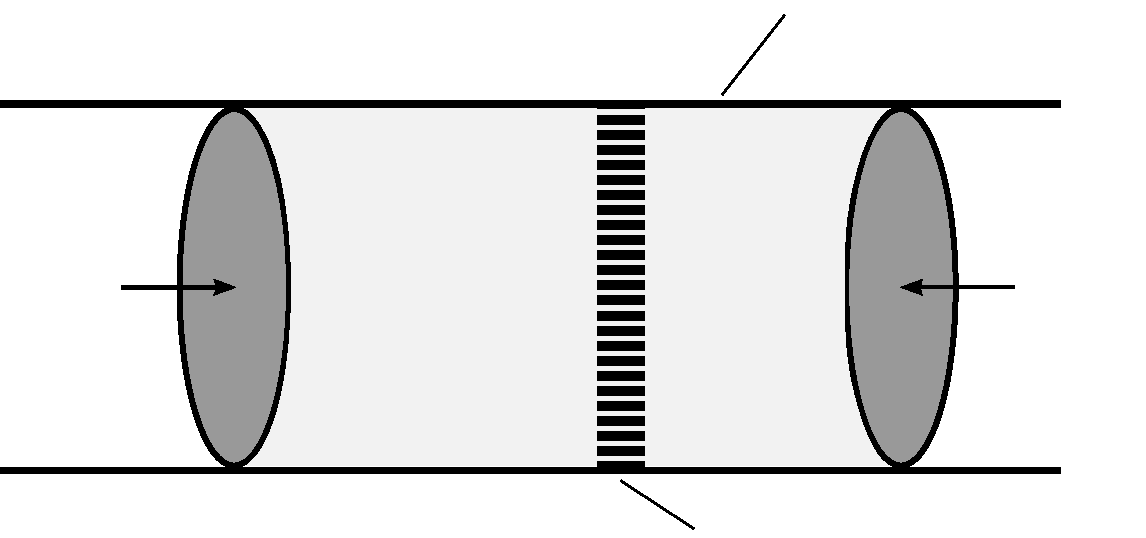
\includegraphics[width=0.3\textwidth]{../img/joule-thomson-process.pdf}
  \caption{Joule-Thomson-Prozess.}
  \label{img:joule-thomson-process}
\end{center}
\end{figure}
Gasströmung bei konstant gehaltenen Druckwerten $p_1, p_2$. Irreversibler Prozess, keine Strömungsenergie wegen Drossel.
\begin{equation}
    \begin{split}
        \difd E &= \difd E_1 + \difd E_2 = - p_1 \difd V_1 - p \difd V_2 \\
        & \overset{p_1, p_2 = \const}{=} - \difd (p_1 V_1) - \difd (p_2, V_2) \\
        & \Rightarrow \difd (E_1 + p_1 V_1) + \difd (E_2 p_2 V_2) = 0
    \end{split}
\end{equation}
$\Rightarrow$ Die Gesamtenthalpie $H = E + p V$ bleibt erhalten.\\
Von Interesse: Temperaturänderung bei Druckänderung. Infinitesimal verrücken.
\begin{equation}
    \frac{\Delta T}{\Delta p} \to \pdi{T}{p}{N, H} \equiv \kappa_\text{JT}
\end{equation}
Berechnung ($N$ konstant)
\begin{equation}
    \begin{split}
     \pdi{T}{p}{H} &= \pd{(T, H)}{(p, H)} = \pd{(T, H)}{(T, p)} \cdot \pd{(T, p)}{(p, H)} \\ 
    &= - \pdi{H}{p}{T} / \pdi{H}{T}{p} \\
    \difd H &= T \difd S + V \difd p = T \pdi{S}{T}{p} \difd T + \left[ T \pdi{S}{p}{T} + V \right] \difd p \\
    & \Rightarrow \pdi{H}{T}{p} = T \pdi{S}{T}{p} = c_p \\
    \pdi{H}{p}{T} &= V + T \pdi{S}{p}{T} = V - T \pdi{V}{T}{p} \text{ (mit Maxwellbeziehung zu $G$)} \\
    &= V \left[ 1 - T \alpha \right]
    \end{split}
\end{equation}
Damit
\begin{equation}
    \kappa_\text{JT} = \frac{V \left( T \alpha - 1 \right) }{c_p}
\end{equation}
Im Versuch ist $\delta p$ negativ (Druckverminderung)
\begin{equation}
    \Rightarrow
    \begin{cases}
        \kappa_\text{JT} > 0 & \text{Temperaturabnahme} \\
        \kappa_\text{JT} < 0 & \text{Temperaturzunahme} \\
    \end{cases}
\end{equation}
\begin{enumerate}[a)]  % TODO alpha
    \item Ideales Gas
    \begin{equation}
        \begin{split}
            \alpha &= \frac{1}{V} \pdi{V}{T}{p} = \frac{1}{V} \frac{N k}{p} = \frac{N k}{N k T} = \frac{1}{T} \\
            & \Rightarrow T \alpha - 1 = 0 \Rightarrow \kappa_\text{JT} = 0
        \end{split}
    \end{equation}
    \item van-der Waals Gas: Hier, i.A. ist $\kappa_\text{JT} \neq 0$ (hängt von $p, T$ ab) \\
    Die Kurve, für die $\kappa_\text{JT} = 0 $ gilt, heißt \emph{Inversionskurve}. Kühleffekte nur innerhalb 
    $\kappa_\text{JT} > 0$
\end{enumerate}

\subsection{Thermodynamische Potentiale}
Bereits kennengelernt $E(S, V, n), F(T, V, N), H(S, p, N), G(T, p, N)$ und Varianten, z.B. $S(E, V, N)$. Die obigen Potentiale
sind durch sogenannte \emph{Legendre-Transformationen} miteinander verknüpft. \\
Allgemeines Schema: Sei $P(x_1, \ldots, x_n)$ ein thermodynamisches Potential mit
\begin{equation}
    \difd P = K_1 \difd x_1 + K_2 \difd x_2 + \ldots + K_n \difd x_n
\end{equation}
Dann ist $Q_i := P - K_i x_i$ neues thermodynamisches Potential mit
\begin{equation}
    \begin{split}
        \difd Q_i &= K_1 \difd x_1 + \ldots + K_i \difd x_i + \ldots + K_n \difd x_n - K_i \difd x_i - x_i \difd K_i \\
        & = K_1 \difd x_1 + \ldots - x_i \difd K_i + \ldots + K_n \difd x_n
    \end{split}
\end{equation}
d.h. $Q_i = Q(x_1, \ldots, x_{i-1}, K_i, x_{i+1}, \ldots, x_n)$ und
\begin{equation}
    \pdi{Q_1}{x_1}{x_2, \ldots, K_i, \ldots, x_n} = K_1, \ldots, \pdi{Q}{K_i}{x_1, \ldots, x_i, \ldots x_n} % TODO letztes x_i durchgestrichen
\end{equation}
Die beiden Potentiale $P$ und $Q$ enthalten die gleichen Information. Es ist eine Frage der Zweckmäßigkeit, welches thermodynamisches Potential
im Spezialfall benutzt wird. \\
$x_1, \ldots, x_i, \ldots, x_n \to $ natürliche Variable von $P$; \\
$x_1, \ldots, k_i, \ldots, x_n \to$ natürliche Variable von $Q_i$ \\
Zum Informationsverlust bei beliebigen Transformationen und zur heuristischen Begründung der Legendre-Transformation siehe z.B. A. u. H. §3.23. \\[\baselineskip]
Damit enthalten $E, F, G$ und $H$ als Funktion ihrer natürlichen Variablen die gleiche INformation
\begin{equation}
    \begin{split}
        & F(T, V, N) = E - ST \\
        & G(T, p, N) = F + p V = E - ST + pV \\
        & H(S, p, N) = E + pV
    \end{split}
\end{equation}
Bedeutung:
\begin{description}
    \item[$F$] \emph{isotherme Prozesse}: Freie Energie; Anteil der Gesamtenergie, der zur Arbeitsleistung verwendet werden kann
    \item[$G$] \emph{isotherm-isobare Prozesse}: Freie Enthalpie (Gibbssches Potential); Wichtig für chemische Prozesse.
    \item[$H$] \emph{adiabatisch-isobare Prozesse}
\end{description}
Es gibt weitere thermodynamische Potentiale, z.B. das \emph{großkanonische} Potential $\Omega = \Omega(T, V, \mu)$. 
\begin{equation}
    \begin{split}
        \Omega(T, V, \mu) &= F - \mu N \\
        \Rightarrow \difd \Omega &= - S \difd T - p \difd V - N \difd \mu
    \end{split}
\end{equation}
Fundamentalbeziehung $F=-pV + \mu N$
\begin{equation}
    \Rightarrow \Omega = - p V
\end{equation}
Vorsicht: $p$ ist \emph{keine} natürliche Variable von $\Omega$; für die Kenntnis des Systems brauchen wir $p(T, V, \mu)$.\\[\baselineskip]
Ein Beispiel zum Zurückrechnen: $\Omega$ ist bekannt; wie sieht $E$ aus? \\
$\Omega(T, V, \mu)$ bekannt:
\begin{equation}
    \begin{split}
        S &= \pdi{\Omega}{T}{V, \mu} \\
        N &= \pdi{\Omega}{\mu}{T, V} \\
        \Rightarrow &
        \begin{cases}
            S(T, V, \mu) \\
            N(T, V, \mu)
        \end{cases} \\
        \Rightarrow &
        \begin{cases}
            T = T(S, V, N) \\
            \mu = \mu(S, V, N)
        \end{cases} \\
        \Rightarrow & E(S, V, N) = \Omega + TS + \mu N \\
        &= \Omega(T(S, V, N), V, \mu(S, V, N)) + T(S, V, N) S + \mu (S, V, N) N
    \end{split}
\end{equation}
\begin{equation}
    \begin{array}{lll}
        E & \difd E = T \difd S - p \difd V + \mu \difd N & E(S, V, N) \\
        F = E - TS & \difd F = - S \difd T - p \difd V + \mu \difd N & F(T, V, N) \\
        H = E + pV & \difd H = T \difd S + V \difd p + \mu \difd N & H(S, p, N) \\
        G = E - TS + pV & \difd G = - S \difd T + V \difd p + \mu \difd N & G(T, p, N) \\
        \Omega = E - TS - \mu N & \difd \Omega = - S \difd T - p \difd V - N \difd \mu & \Omega(T, V, \mu)
    \end{array}
\end{equation}
Es gibt noch weitere zwei thermodynamische Potentiale, welche allerdings ungebräuchlich sind.